In this section, we shall describe a model for simulating the erosion of a stone. In particular, we think of the erosion of a stone as coming from shear forces. This discrete model for eroding the stone allows us to simulate random processes and view the shape of a stone after some number of time steps. We provide computer simulations for the erosion process and analyze the model through these simulations.

\subsection{Shearing Stones}

The discrete model for stone erosion is based on the idea that stones are eroded via chipping. The process of chipping is analogous to dropping a stone from a specified height and applying a shear force to a particular point on the stone. Intuitively, one can think of a stone in a stream being eroded by being tossed and turned by the force of the river. This tossing and turning causes the stone to collide with other stones on the bottom of the riverbed, causing chipping to occur.

We model the interaction between two stones as a shear force - a force that causes two parts of a stone to move in opposite directions. The point where a stone collides with another stone is the point where the shear force is concentrated. This causes the stone to break into two pieces. In mechanics, the shear stress $\tau$ applied to the stone is given by the following equation:

\begin{eqnarray}
  \tau = \frac{F}{A}
\end{eqnarray}

Where $F$ is the force applied and $A$ is the cross-sectional area of material with area parallel to the applied force vector. If the shear stress $\tau$ is above the stress that the stone's material can withstand, then the stone will crack.

Notice that the stress is proportional to the cross-sectional area of meterial which is parallel to the force vector. Thus, we can see that if the amount of force applied is constant, the total area of the material that will be sheared if shearing occurs will be constant as well.

\subsection{Definitions}

This section will define how we represent a stone in the discrete model.

We will represent a stone as a polygon with $n$ vertices. Formally, a polygon $s$ can be defined as the set of vertices $s = \{ \bvec{v}_1, \ldots, \bvec{v}_n \}$, where a vertex $\bvec{v}_i = (x_i, y_i)$ is a tuple in $\mathrm{R}^2$. In a polygon $s$, vertices $\bvec{v}_i$ and $\bvec{v}_{i+1}$ are connected by a line segment for $i \in \{1,2, \ldots, n-1\}$. In addition, vertices $\bvec{v}_{n}$ and $\bvec{v}_1$ are also connected by a line segment.

The centroid $\bvec{c}_s$ of a stone $s$ is the center of mass of the stone when the stone has uniform density. In other words, the centroid is the point $\bvec{c}_s \in \mathrm{R}^2$ where the following holds:

\begin{eqnarray}
 \int_A (\bvec{r} - \bvec{c}_s) dA = 0
\end{eqnarray}

Where $A$ is the area of the stone.

\subsection{The Chipping Process Model}

With this in mind, we shall now develop a model for the erosion of a stone based on shearing. The main idea of the model is that we will represent a stone as a two-dimensional polygon, and chip off a constant amount of area of the stone at every time step. In this way, we will attempt to capture the process of a stone colliding with another stone on a riverbed. Randomness will be introduced into the model by randomly selecting somewhere on the stone to start the shearing.

We shall now give a formal definition of the chipping process. A chip for a probability distribution $\mathrm{P}$, stone $s$, and area $A$ is denoted $Chip(\mathrm{P}, A, s)$ and is represented as follows:

\begin{enumerate}
  \item Select a vertex $\bvec{v}_j$ from $s$. To select this vertex, we find the centroid $\bvec{c}_s$ of stone $s$ and choose an angle $\gamma \in [0, 2\pi)$ uniformly at random. Now, define the ray $\bvec{l}$ as the ray with an initial point of $\bvec{c}_s$ which extends outwards infinitely at an angle of $\gamma$ from the horizontal. The vertex with the minimum perpendicular distance to $\bvec{l}$ will be $\bvec{v}_j$.
  \item Given vertex $\bvec{v}_j$, define $\bvec{l}_1$ as the line segment which connects $\bvec{v}_j$ and $\bvec{v}_{{j-1} \pmod{n}}$. Similarly, define $\bvec{l}_2$ as the line segment connecting $\bvec{v}_j$ and $\bvec{v}_{{j+1} \pmod{n}}$.
  \item Select a point $\bvec{p}_1$ at random from $\bvec{l}_1$. To do this, we select a random $t \in [0,1]$ such that $\bvec{p}_1 = \bvec{v}_j t + (1-t) \bvec{v}_{{j-1} \pmod{n}}$. The distribution of $t$ is defined by the probability distribution $\mathrm{P}$ so that $t \sim \mathrm{P}$.
  \item Select the point $\bvec{p}_2$ which lies on $\bvec{l}_2$ for which the polygon defined by $\{\bvec{p}_1, \bvec{v}_j, \bvec{p}_2\}$ has an area of $A$. If no such polygon exists, then choose $\bvec{p}_2 = \bvec{v}_{{j+1} \pmod{n}}$.
  \item Create a new stone $s'$ whose vertices are given by $s' = \{ \bvec{v}_1, \ldots, \bvec{v}_{j-1}, \bvec{p}_1, \bvec{p}_2, \bvec{v}_{j+1}, \ldots, \bvec{v}_n \}$. Here, the vertex $\bvec{v}_j$ has been replaced by $\bvec{p}_1$ and $\bvec{p}_2$ in the list of vertices for $s$. The new stone $s'$ now has one more line segment and vertex than the old stone $s$.
\end{enumerate}

A chipping process for a probability distribution $\mathrm{P}$, stone $s$, area $A$, and iterations $k$ is denoted $ChipProcess(\mathrm{P}, A, s, k)$. A chipping process returns a stone $s'$ which has iteratively been through $k$ chips. Thus, a chipping process takes a stone $s$ and creates $s_1 = Chip(\mathrm{P}, A, s)$, $s_2 = Chip(\mathrm{P}, A, s_1)$, \ldots, $s_k = Chip(\mathrm{P}, A, s_{k-1})$, and returns $s' = s_k$.

\subsection{Simulations}

The chipping process model allows us to simulate changes to a stone. A stone which undergoes a chipping process should have a shape which is close to the stones which undergo erosion and chipping in the real world (if our chipping process model is an accurate description of erosion).

To examine the accuracy of our model, we performed computer simulations using the Python programming language and the Shapely library. With computer simulations, we were able to create multiple instances of a chipping process and analyze the shapes of the resulting stones. We were also able to use multiple probability distributions $\mathrm{P}$ and areas $A$ to generate different chipping processes.

\begin{figure}[H]
  \begin{center}
    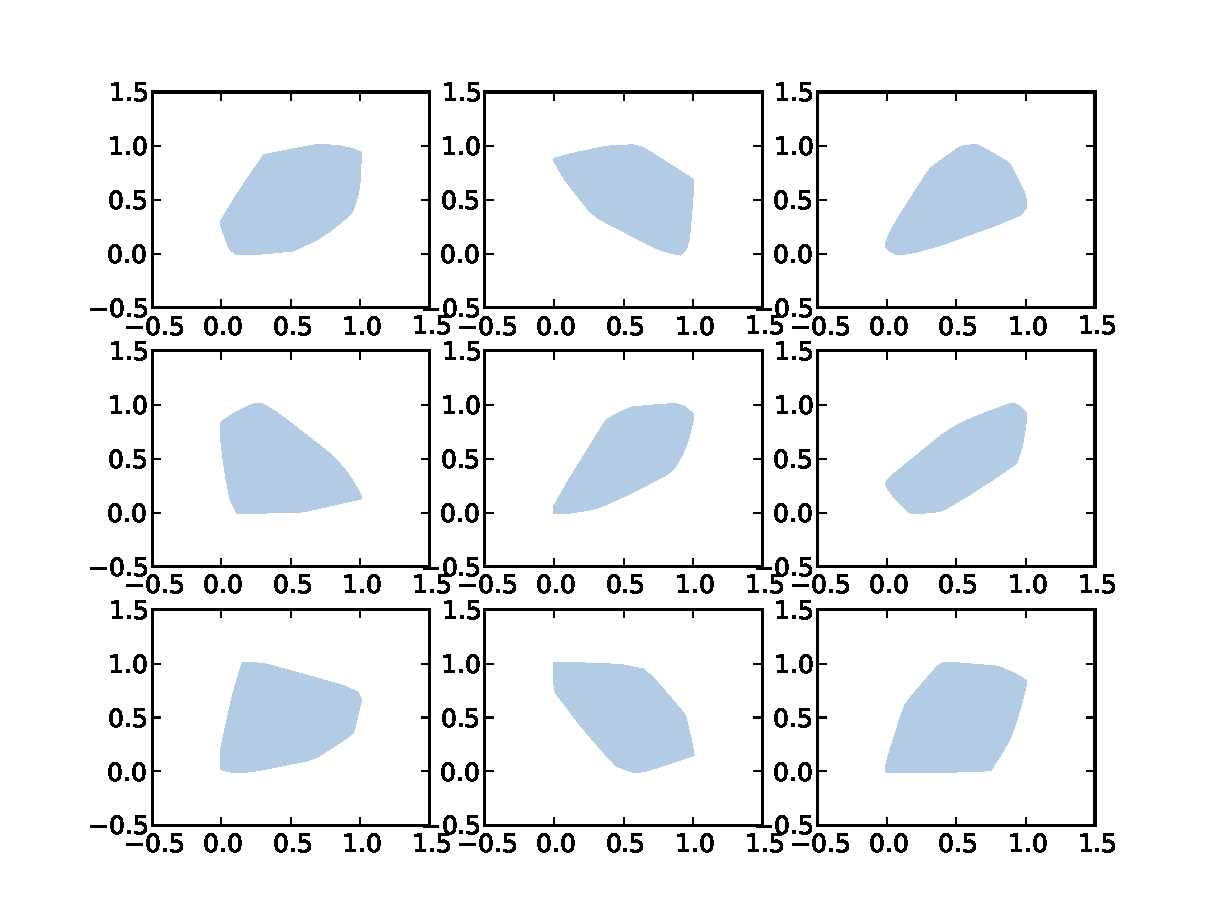
\includegraphics[width=4in]{area_chipper_sample.pdf}
  \end{center}
  \label{fig:area_chipper_sample}
  \caption{Chipping Process for a Unit Square}
\end{figure}

Figure \ref{fig:area_chipper_sample} shows the results for nine chipping process runs. The parameters used in these runs were $\mathrm{P} = \mathrm{N}(0.5, 0.15)$, $A = 0.05$, $k = 50$, and $s = \{(0,0), (1,0), (1,1), (0,1)\}$. The chipping processes each started out with a stone which was a unit square. The stones were chipped 50 times by the method described by the model. The probability distribution $\mathrm{P}$ is a normal distribution so that $t = 0.5$ is the most likely $t$ to choose. In other words, it is most likely that $\bvec{p}_1$ will be chosen as the midpoint of the line segment $\bvec{l}_1$.

This distribution was chosen because it is more likely that shear forces will cause a symmetric split about the vertex $\bvec{v}_j$. However, it is still possible for non-symmetric splits to occur, i.e. when $t \neq 0.5$. The normal distribution captures this nicely (all realizations of $t$ which are not in the interval $[0,1]$ were discarded).

Figure \ref{fig:area_chipper_sample} displays the typical results of the chipping process model. None of the stones resemble a square and it would be hard for anyone to have guessed that these shapes came from a common origin. In fact, the randomization from the distribution $\mathrm{P}$ makes all of the shapes slightly different.

To examine the chipping process more closely, we can look at how circular or elliptical the resulting shapes are. One would expect rocks in a stream or riverbed to be elliptical in shape. We can therefore examine the distance of each vertex from the centroid of the stone. In a circle, all of the distances would be the same. In an elipse, one would expect to have an even number of points which are close and far away.

\begin{figure}[H]
  \begin{center}
    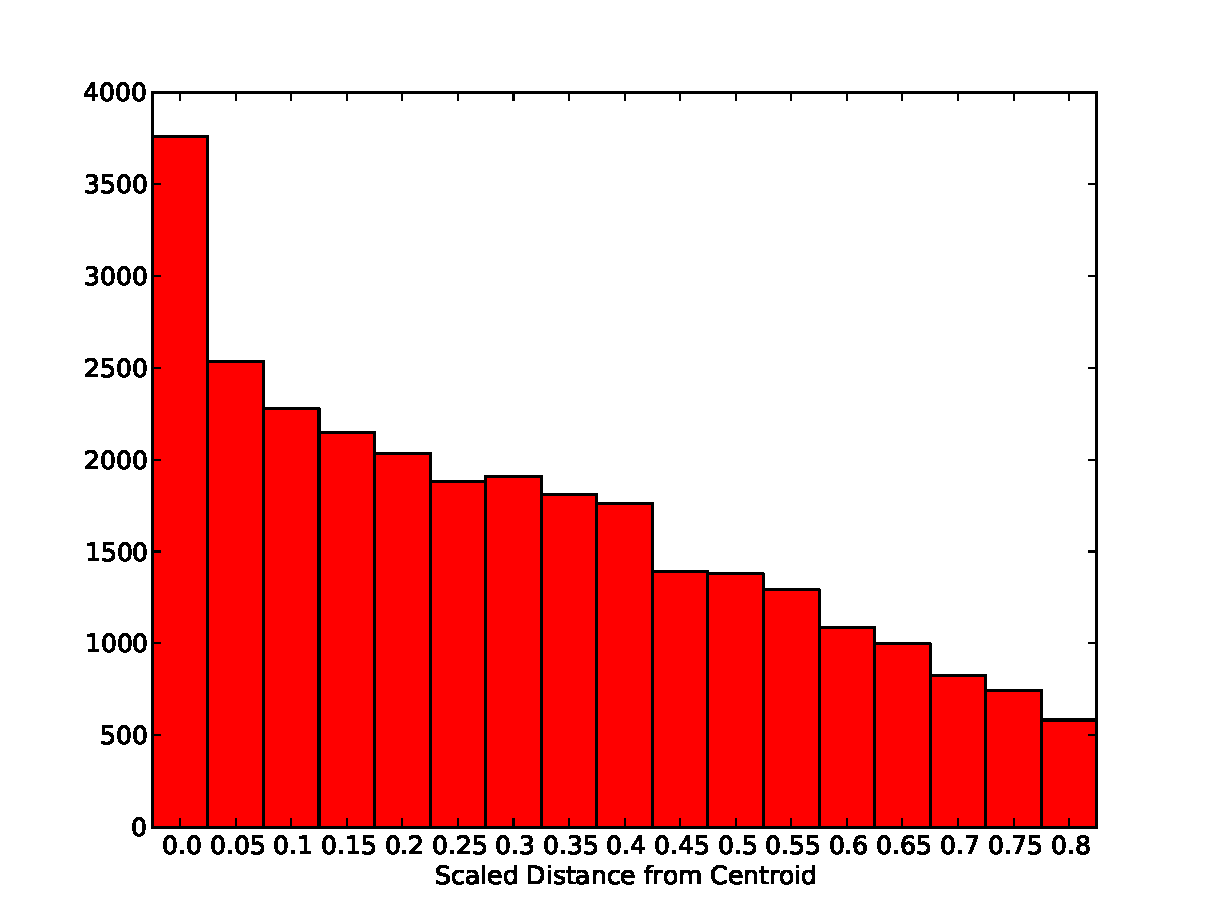
\includegraphics[width=4in]{distance_from_centroid.pdf}
  \end{center}
  \label{fig:distance_from_centroid}
  \caption{Histogram of Vertex Distance From Centroid}
\end{figure}

Figure \ref{fig:distance_from_centroid} shows the distribution of vertex distances which were simulated with the same parameters as used for figure \ref{fig:area_chipper_sample}. One can see that the distribution looks fairly normal, with a mean of a distance of 0.472. The distribution of vertex distances from the centroid show that the shapes that result from this set of chipping process conditions are neither elliptical nor spherical. However, a probability distribution $\mathrm{P} = \mathrm{N}(0.5, 0.15)$ tends to create a distribution of vertex distances from the centroid which are normal.

Choosing a different distribution for $\mathrm{P}$ yields dramatically different results. For example, if we choose $\mathrm{P} = \mathrm{N}(0.05, 0.15)$, we obtain the distribution shown in figure \ref{fig:distance_from_centroid_skewed}.

\begin{figure}[H]
  \begin{center}
    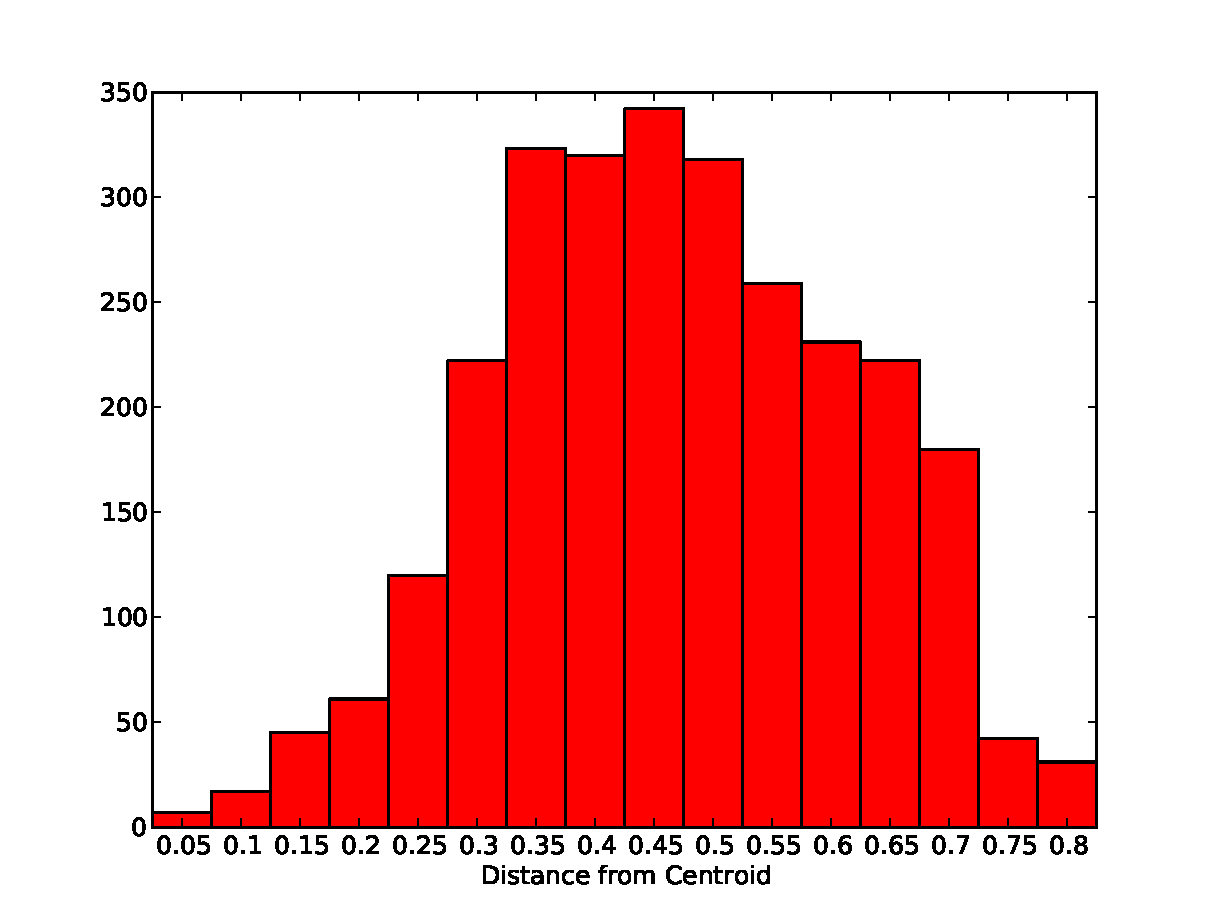
\includegraphics[width=4in]{distance_from_centroid_skewed.pdf}
  \end{center}
  \label{fig:distance_from_centroid_skewed}
  \caption{Histogram of Vertex Distance From Centroid for $\mathrm{P} = \mathrm{N}(0.05, 0.15)$}
\end{figure}

One can see that the distribution of vertex distances from the centroid are skewed so that there are far more vertices which are further away from the centroid. The resulting stones are much flatter than the stones shown in figure \ref{fig:area_chipper_sample}. The intuitive explanation for this is that there is a much higher probability that the shear will not be symmetric, so that the area that is removed will be much thinner. Because of this, it is more likely that longer, thinner stones will result.
